\chapter{Fit for $F_{+}(hh\pi^0)$}

The fit was done on the data emailed by Chris:
\begin{table}[!h]
	\begin{center}
		\begin{tabular}{c| c|c|c|c}
			bin & PiPiPi0 vs KsPiPi & PiPiPi0 vs KlPiPi & KKPi0 vs KsPiPi & KKPi0 vs KlPiPi  \\
			\hline
			\hline
1 & $201.4 \pm 37.0$ & $377.8 \pm 45.9$ & $81.3 \pm 23.9$ & $86.8 \pm 24.2$ \\
2 & $117.0 \pm 29.0$ & $142.2 \pm 28.3$ & $28.4 \pm 14.7$ & $38.6 \pm 16.7$ \\
3 & $162.9 \pm 31.0$ & $138.9 \pm 29.2$ & $40.1 \pm 16.1$ & $15.2 \pm 14.3$ \\
4 & $114.4 \pm 26.1$ & $29.8 \pm 15.6$ & $10.9 \pm 8.4$ & $2.7 \pm 7.9$ \\
5 & $573.9 \pm 60.9$ & $24.3 \pm 20.8$ & $47.1 \pm 19.5$ & $-2.7 \pm 16.2$ \\
6 & $183.1 \pm 34.7$ & $55.7 \pm 19.6$ & $26.6 \pm 13.8$ & $38.1 \pm 15.9$ \\
7 & $206.2 \pm 37.3$ & $197.1 \pm 32.1$ & $46.4 \pm 18.0$ & $75.7 \pm 20.7$ \\
8 & $196.4 \pm 35.6$ & $277.6 \pm 39.1$ & $38.7 \pm 16.5$ & $87.2 \pm 22.5$ \\ 
\end{tabular}
\end{center}
\caption{\textit{$M_i + M_{-i}$ for $hh\pi^0$ vs \KsPiPi and \KlPiPi.}}
\end{table}


\section{$\pi \pi \pi^0$}
\begin{table}[!h]
	\begin{center}
		\begin{tabular}{c| c|c|c}
			 & $\pi \pi \pi^0$ vs \KsPiPi & $\pi \pi \pi^0$ vs \KlPiPi & simultaneous \\
			\hline
			\hline
			$F_+$ &  1.001 $\pm$ 0.054 & 0.992 $\pm$ 0.081 & 0.999 $\pm$ 0.045 \\
			$h_{\KsPiPi}$ & 933.471 $\pm$ 61.130 & --- &  933.636 $\pm$ 60.656 \\
			$h_{\KlPiPi}$ & --- & 497.190 $\pm$ 44.564 & 494.871 $\pm$ 48.840 \\
			$\chi^2_{ndof}$ & 0.422 & 0.232 &  0.330 \\
\end{tabular}
\end{center}
\caption{\textit{Results of the fit for $F_+$ in $\pi \pi \pi^0$.}}
\end{table}
\clearpage
\begin{figure}[!h]
	\vspace*{-0.5cm}
	\begin{center}
	\subfigure{ 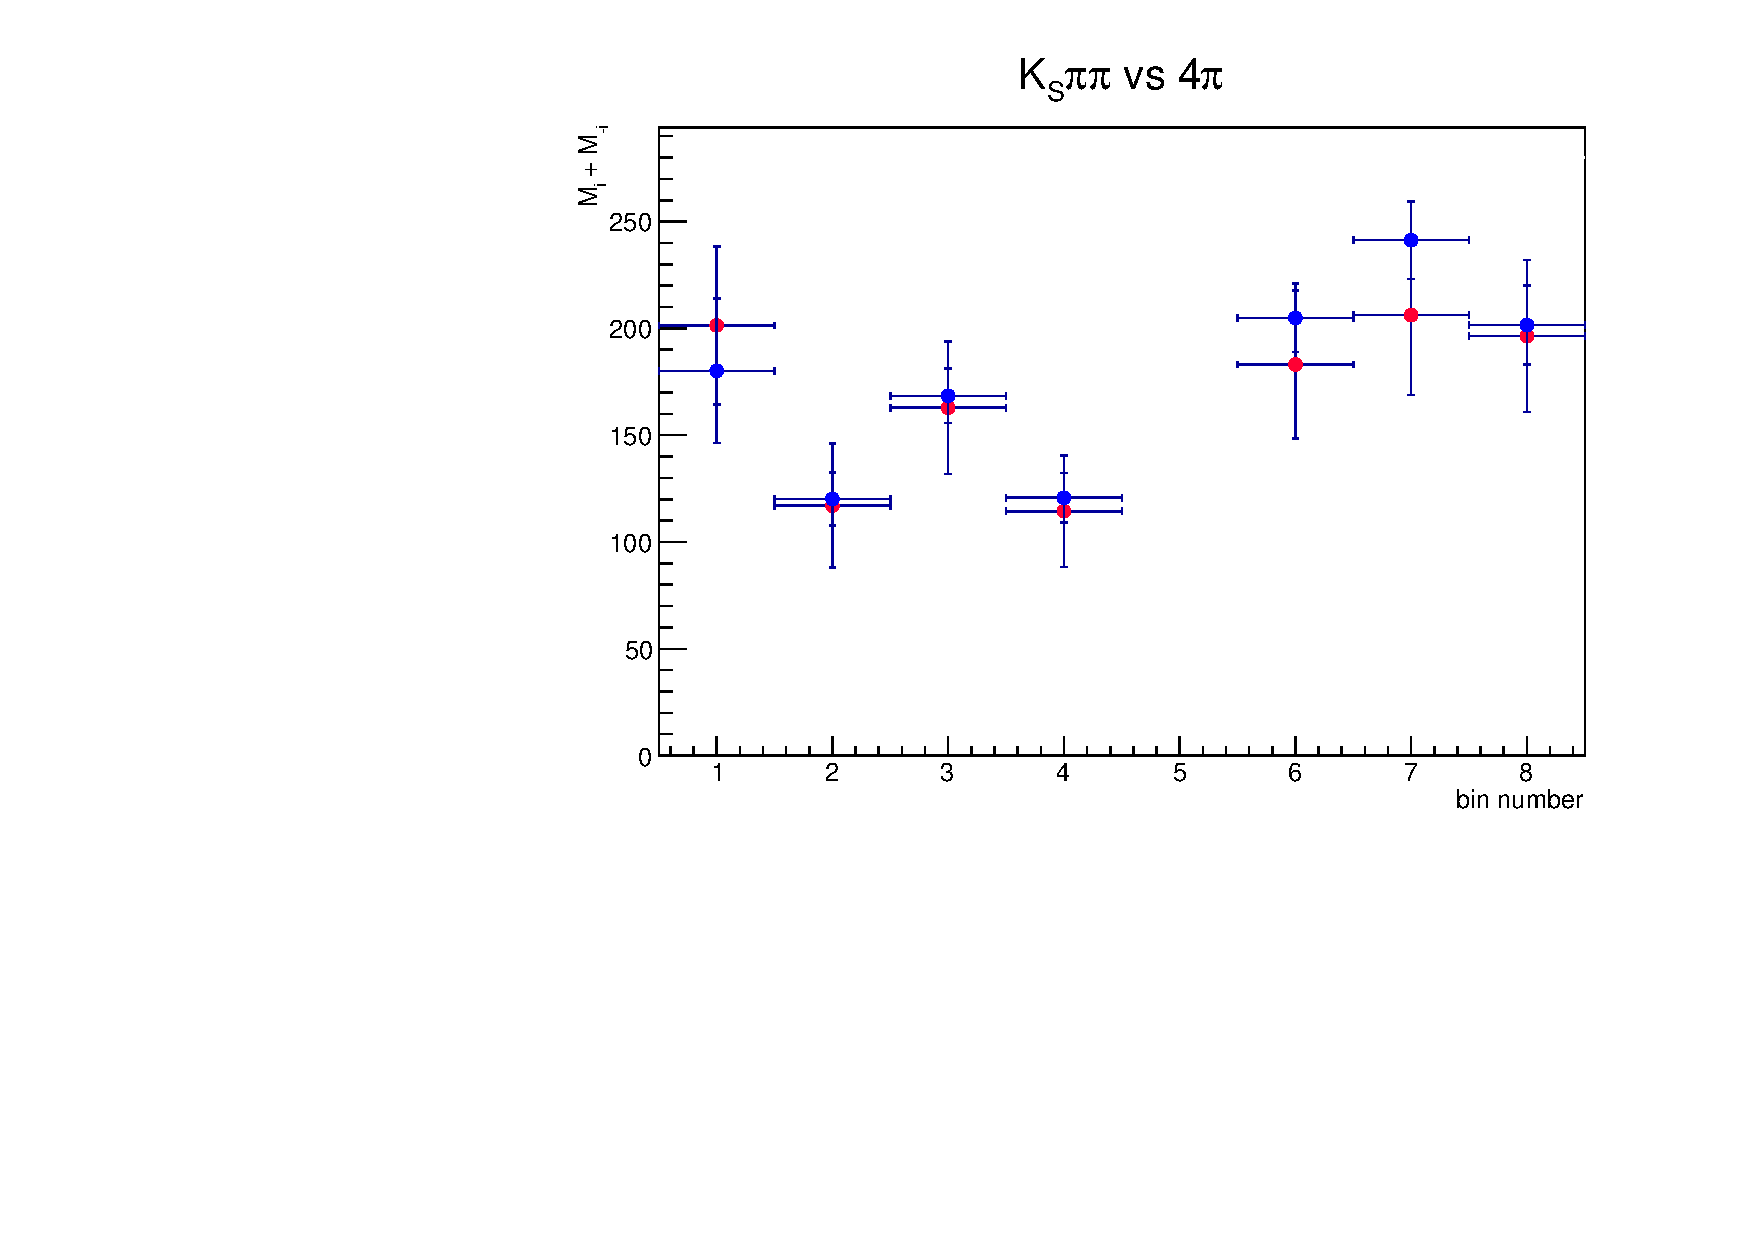
\includegraphics[width=0.48 \textwidth] {F_pipipi0_KsPiPi.pdf}}
	\subfigure{ 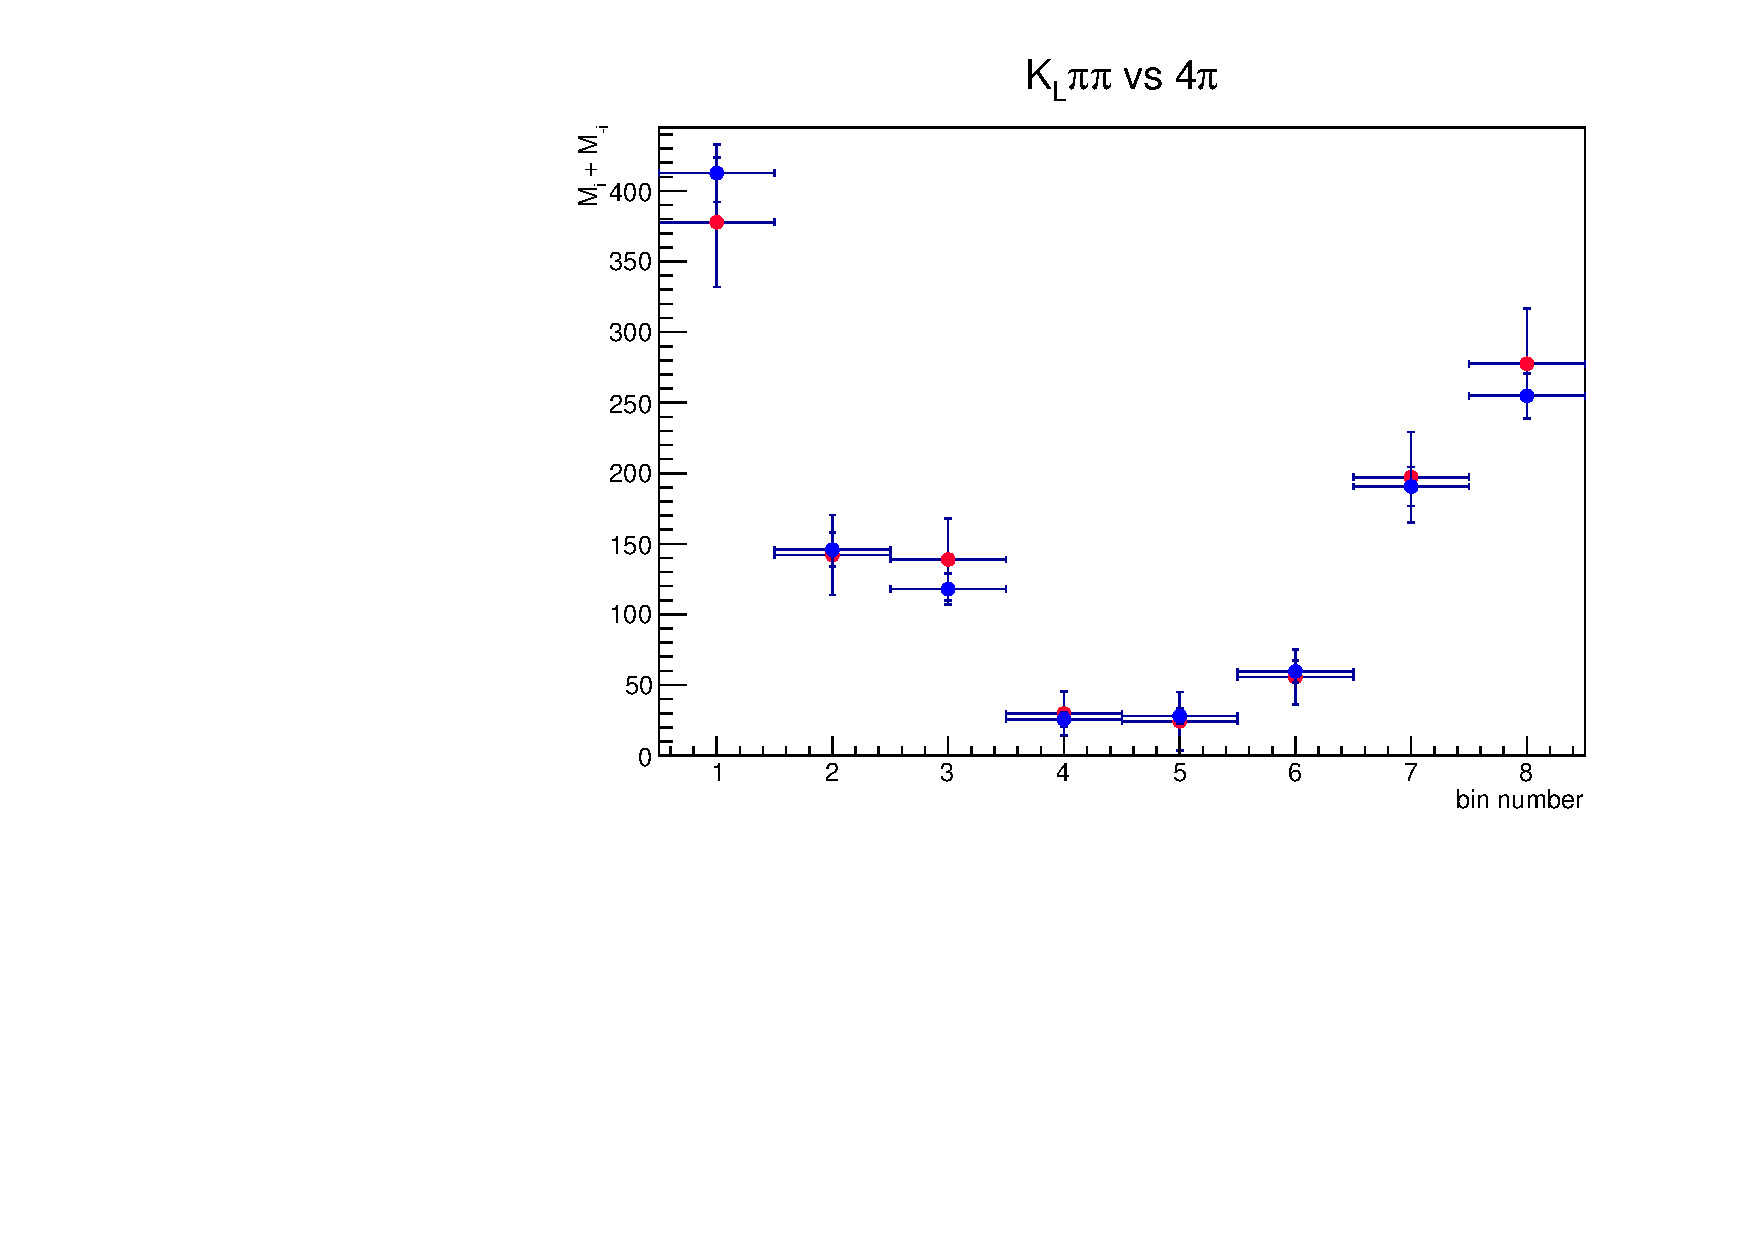
\includegraphics[width=0.48 \textwidth] {F_pipipi0_KlPiPi.pdf}}
		\vspace*{-0.5cm}
	\end{center}
	\caption{\textit{Distribution of $MM$ over the bins for $\pi \pi \pi^0$ vs \KsPiPi (left) and $\pi \pi \pi^0$ vs \KlPiPi (right). The fit was performed on both modes independently of each other. Red: data, blue: fit values. }}
\end{figure}\\


\begin{figure}[!h]
	\vspace*{-0.5cm}
	\begin{center}
	 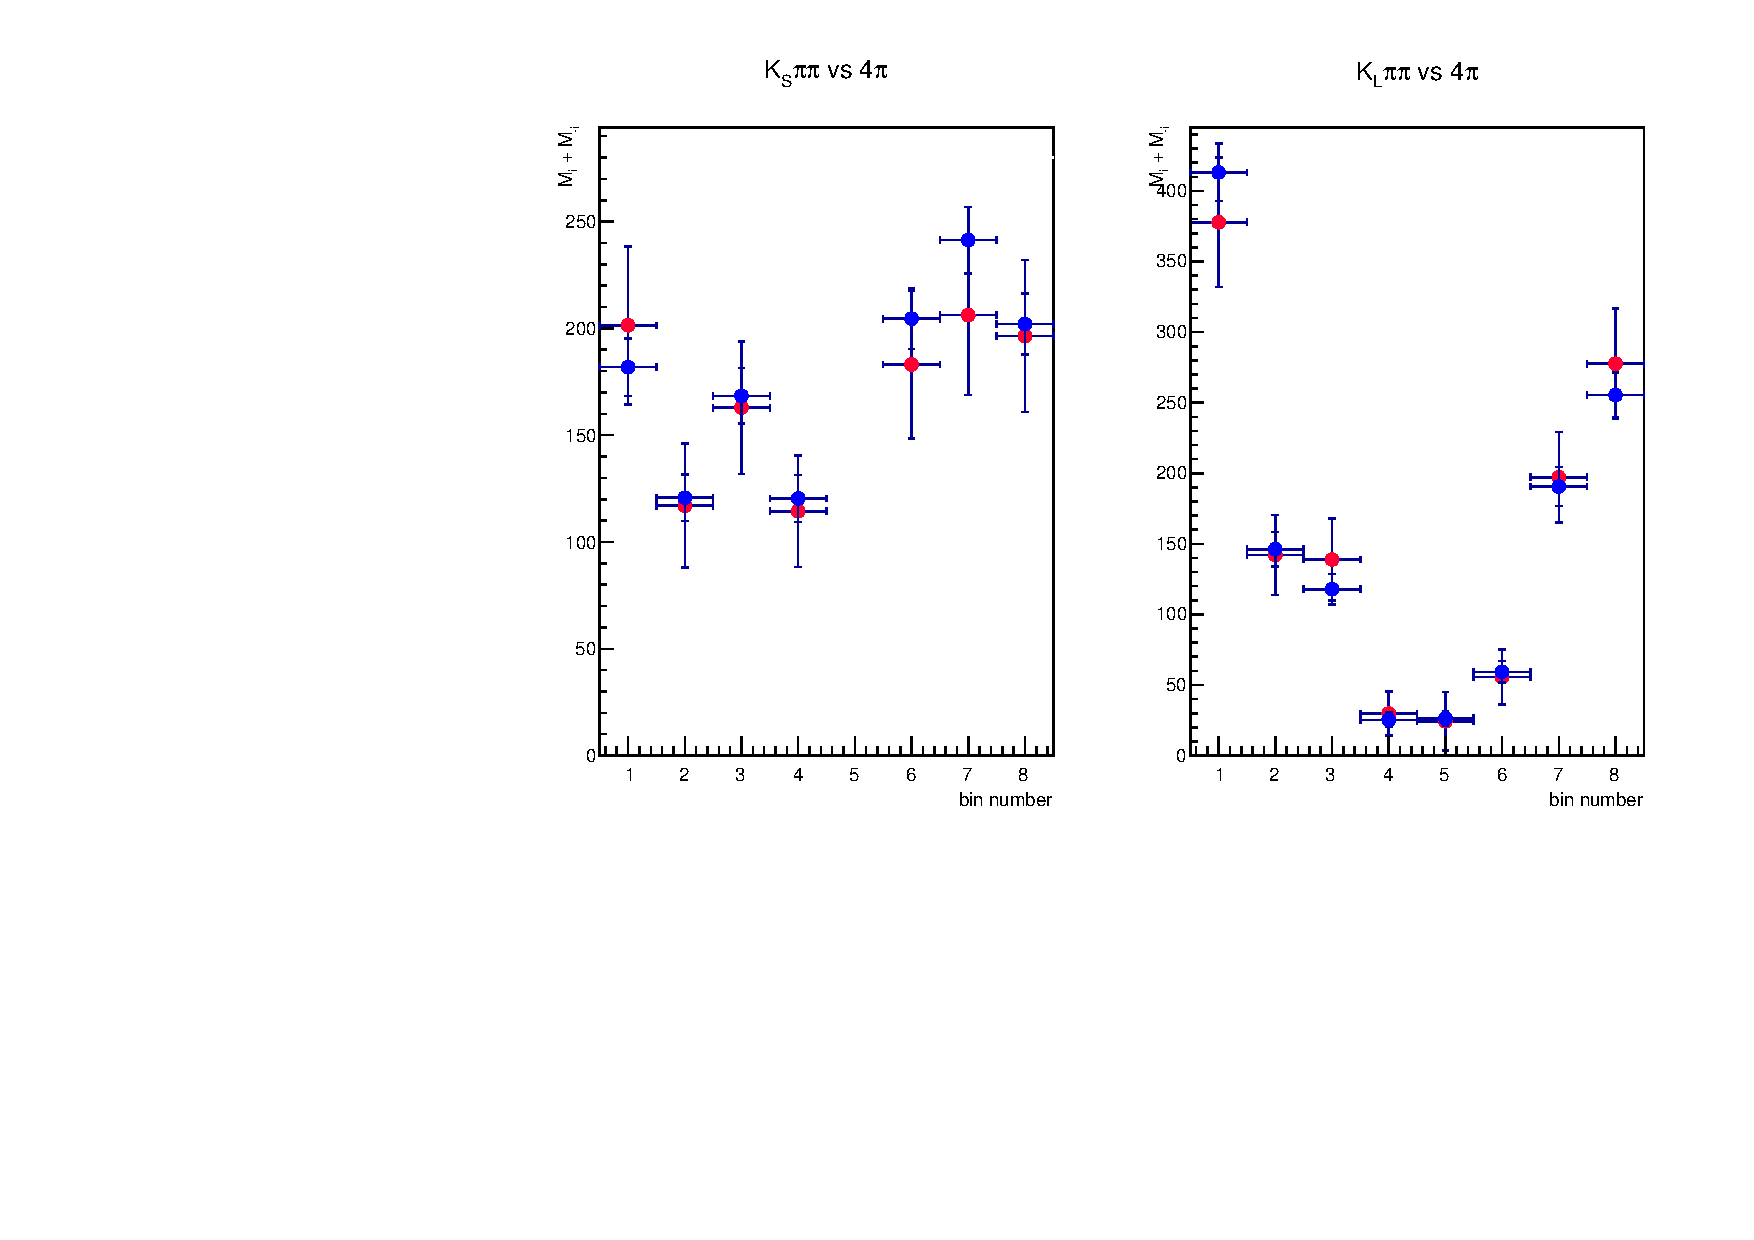
\includegraphics[width=0.96 \textwidth] {F_pipipi0_both.pdf}
		\vspace*{-0.5cm}
	\end{center}
	\caption{\textit{Distribution of $MM$ over the bins for $\pi \pi \pi^0$ vs \KsPiPi (left) and $\pi \pi \pi^0$ vs \KlPiPi (right). The fit was performed on both modes simultaneously. Red: data, blue: fit values. }}
\end{figure}\\
\clearpage
\subsection{Change in input variables}
\begin{table}[!h]
	\begin{center}
		\begin{tabular}{c| c| c|c}
			input variable & \quad shift [\%] \quad & shift/$\sigma_{fit}$ & \quad $\sigma_{fit}/ \sigma_{input}$\\
			\hline
			\hline
$c_1$ & 0.14 & 0.046 & 0.35\\ 
$c_2$ & 0.58 & 0.096 & 0.33\\ 
$c_3$ & 18 & 0.11 & 0.24\\ 
$c_4$ & -0.82 & 0.087 & 0.35\\ 
$c_5$ & -0.054 & 0.022 & 0.36\\ 
$c_6$ & -0.74 & 0.12 & 0.3\\ 
$c_7$ & 10 & 0.19 & 0.33\\ 
$c_8$ & 0.92 & 0.12 & 0.33\\ 
$T_1$ & 0.26 & 0.084 & 1\\ 
$T_2$ & -0.0084 & -0.0063 & 1\\ 
$T_3$ & -0.056 & -0.021 & 0.99\\ 
$T_4$ & -0.11 & -0.027 & 0.99\\ 
$T_5$ & 0.44 & 0.16 & 0.99\\ 
$T_6$ & -0.088 & -0.048 & 1\\ 
$T_7$ & -0.12 & -0.082 & 1\\ 
$T_8$ & -0.021 & -0.013 & 1\\ 
$T_{-1}$ & 0.00034 & 0.0002 & 1\\ 
$T_{-2}$ & 0.00014 & 0.00013 & 1\\ 
$T_{-3}$ & -0.0051 & -0.0032 & 1\\ 
$T_{-4}$ & -0.45 & -0.047 & 0.99\\ 
$T_{-5}$ & 0.27 & 0.11 & 1\\ 
$T_{-6}$ & -0.047 & -0.023 & 1\\ 
$T_{-7}$ & -0.04 & -0.013 & 1\\ 
$T_{-8}$ & -0.0016 & -0.00044 & 1\\ 
\end{tabular}
\end{center}
\caption{\textit{Amount by which the Gaussian constraint input variables are shifted in the fit with the \KsPiPi mode only.}}
\end{table} 
\clearpage
\begin{table}[!h]
	\begin{center}
		\begin{tabular}{c| c| c|c}
			input variable & \quad shift [\%] \quad & shift/$\sigma_{fit}$ & \quad $\sigma_{fit}/ \sigma_{input}$\\
			\hline
			\hline
$c'_1$ & -0.11 & -0.034 & 0.38\\ 
$c'_2$ & -0.12 & -0.018 & 0.39\\ 
$c'_3$ & 3.4 & 0.13 & 0.46\\ 
$c'_4$ & -0.89 & 0.051 & 0.45\\ 
$c'_5$ & 0.077 & -0.018 & 0.47\\ 
$c'_6$ & 1.1 & -0.035 & 0.45\\ 
$c'_7$ & 1.1 & 0.073 & 0.48\\ 
$c'_8$ & 0.47 & 0.08 & 0.39\\ 
$T'_1$ & -0.25 & -0.1 & 1\\ 
$T'_2$ & -0.082 & -0.019 & 0.99\\ 
$T'_3$ & 0.43 & 0.089 & 0.99\\ 
$T'_4$ & 0.16 & 0.021 & 1\\ 
$T'_5$ & -0.03 & -0.0082 & 1\\ 
$T'_6$ & -0.061 & -0.018 & 1\\ 
$T'_7$ & 0.056 & 0.023 & 1\\ 
$T'_8$ & 0.15 & 0.061 & 1\\ 
$T'_{-1}$ & -11 & -0.65 & 0.9\\ 
$T'_{-2}$ & -1 & -0.051 & 0.95\\ 
$T'_{-3}$ & 3.9 & 0.21 & 0.96\\ 
$T'_{-4}$ & 0.71 & 0.034 & 0.99\\ 
$T'_{-5}$ & -0.074 & -0.0031 & 0.99\\ 
$T'_{-6}$ & -0.53 & -0.023 & 0.99\\ 
$T'_{-7}$ & 0.58 & 0.041 & 0.98\\ 
$T'_{-8}$ & 6.2 & 0.29 & 0.92\\ 
\end{tabular}
\end{center}
\caption{\textit{Amount by which the Gaussian constraint input variables are shifted in the fit with the \KlPiPi mode only.}}
\end{table} 
\clearpage
\begin{table}[!h]
	\begin{center}
		\begin{tabular}{c| c| c|c}
			input variable & \quad shift [\%] \quad & shift/$\sigma_{fit}$ & \quad $\sigma_{fit}/ \sigma_{input}$\\
			\hline
			\hline
$c_1$ & 0.1 & 0.039 & 0.32\\ 
$c_2$ & 0.46 & 0.087 & 0.29\\ 
$c_3$ & 20 & 0.14 & 0.22\\ 
$c_4$ & -1.1 & 0.13 & 0.32\\ 
$c_5$ & -0.11 & 0.049 & 0.34\\ 
$c_6$ & -0.75 & 0.13 & 0.28\\ 
$c_7$ & 11 & 0.21 & 0.32\\ 
$c_8$ & 1.1 & 0.14 & 0.3\\ 
$c'_1$ & 0.041 & 0.014 & 0.35\\ 
$c'_2$ & 0.39 & 0.071 & 0.34\\ 
$c'_3$ & 3.7 & 0.15 & 0.43\\ 
$c'_4$ & -1.4 & 0.081 & 0.44\\ 
$c'_5$ & -0.006 & 0.0014 & 0.46\\ 
$c'_6$ & -0.31 & 0.01 & 0.43\\ 
$c'_7$ & 1.6 & 0.1 & 0.49\\ 
$c'_8$ & 0.9 & 0.16 & 0.38\\ 
$T_1$ & 0.25 & 0.081 & 0.99\\ 
$T_2$ & -0.0098 & -0.0073 & 1\\ 
$T_3$ & -0.056 & -0.021 & 0.99\\ 
$T_4$ & -0.11 & -0.026 & 0.99\\ 
$T_5$ & 0.43 & 0.16 & 0.99\\ 
$T_6$ & -0.087 & -0.048 & 1\\ 
$T_7$ & -0.12 & -0.082 & 1\\ 
$T_8$ & -0.022 & -0.014 & 1\\ 
$T_{-1}$ & 0.0022 & 0.0013 & 1\\ 
$T_{-2}$ & 0.00021 & 0.0002 & 1\\ 
$T_{-3}$ & -0.005 & -0.0032 & 1\\ 
$T_{-4}$ & -0.42 & -0.045 & 0.99\\ 
$T_{-5}$ & 0.27 & 0.11 & 1\\ 
$T_{-6}$ & -0.046 & -0.023 & 1\\ 
$T_{-7}$ & -0.038 & -0.012 & 1\\ 
$T_{-8}$ & -0.0014 & -0.00038 & 1\\ 
$T'_1$ & -0.25 & -0.1 & 1\\ 
$T'_2$ & -0.088 & -0.02 & 0.99\\ 
$T'_3$ & 0.44 & 0.089 & 0.99\\ 
$T'_4$ & 0.18 & 0.023 & 1\\ 
$T'_5$ & -0.01 & -0.0028 & 1\\ 
$T'_6$ & -0.054 & -0.016 & 1\\ 
$T'_7$ & 0.056 & 0.023 & 1\\ 
$T'_8$ & 0.14 & 0.06 & 1\\ 
$T'_{-1}$ & -11 & -0.66 & 0.89\\ 
$T'_{-2}$ & -1.1 & -0.055 & 0.95\\ 
$T'_{-3}$ & 4 & 0.21 & 0.96\\ 
$T'_{-4}$ & 0.77 & 0.037 & 0.99\\ 
$T'_{-5}$ & -0.02 & -0.0008 & 1\\ 
$T'_{-6}$ & -0.46 & -0.019 & 0.99\\ 
$T'_{-7}$ & 0.59 & 0.042 & 0.98\\ 
$T'_{-8}$ & 6.1 & 0.29 & 0.92\\ 
\end{tabular}
\end{center}
\caption{\textit{Amount by which the Gaussian constraint input variables are shifted in the fit with the \KsPiPi and \KlPiPi mode simultaneously.}}
\end{table} 

\clearpage

\section{$\kaon \kaon \pi^0$}
\begin{table}[!h]
	\begin{center}
		\begin{tabular}{c| c|c|c}
			 & $\kaon \kaon \pi^0$ vs \KsPiPi & $\kaon \kaon \pi^0$ vs \KlPiPi & simultaneous \\
			\hline
			\hline
			$F_+$ &  0.539 $\pm$ 0.153 & 1.055 $\pm$ 0.237 &  0.747 $\pm$ 0.111 \\
			$h_{\KsPiPi}$ & 157.035 $\pm$ 24.108 & --- &   155.592 $\pm$ 24.549 \\
			$h_{\KlPiPi}$ & --- & 125.350 $\pm$ 26.758 &  146.618 $\pm$ 23.519 \\
			$\chi^2_{ndof}$ & 0.168 & 0.971 &  0.824 \\
\end{tabular}
\end{center}
\caption{\textit{Results of the fit for $F_+$ in $\pi \pi \pi^0$.}}
\end{table}

\begin{figure}[!h]
	\vspace*{-0.5cm}
	\begin{center}
	\subfigure{ 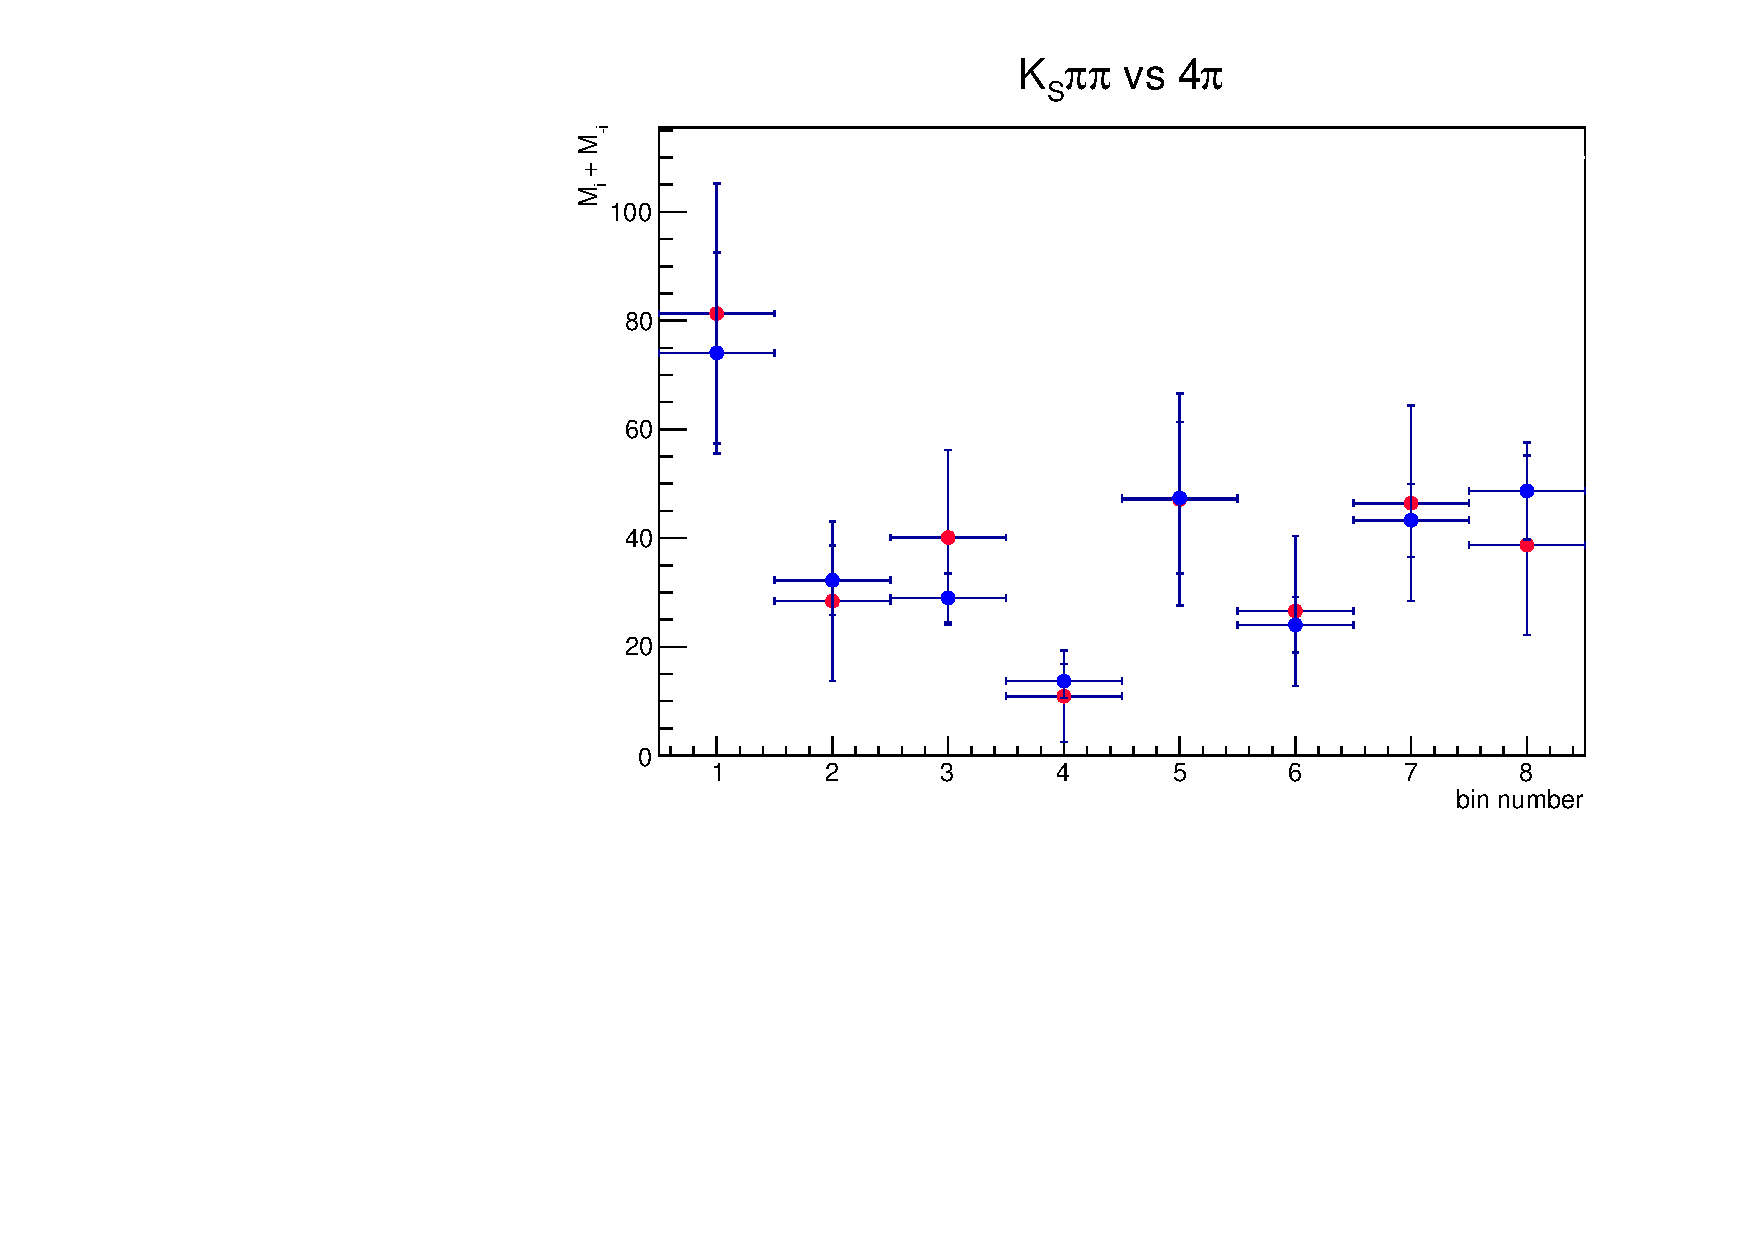
\includegraphics[width=0.48 \textwidth] {F_KKpi0_KsPiPi.pdf}}
	\subfigure{ 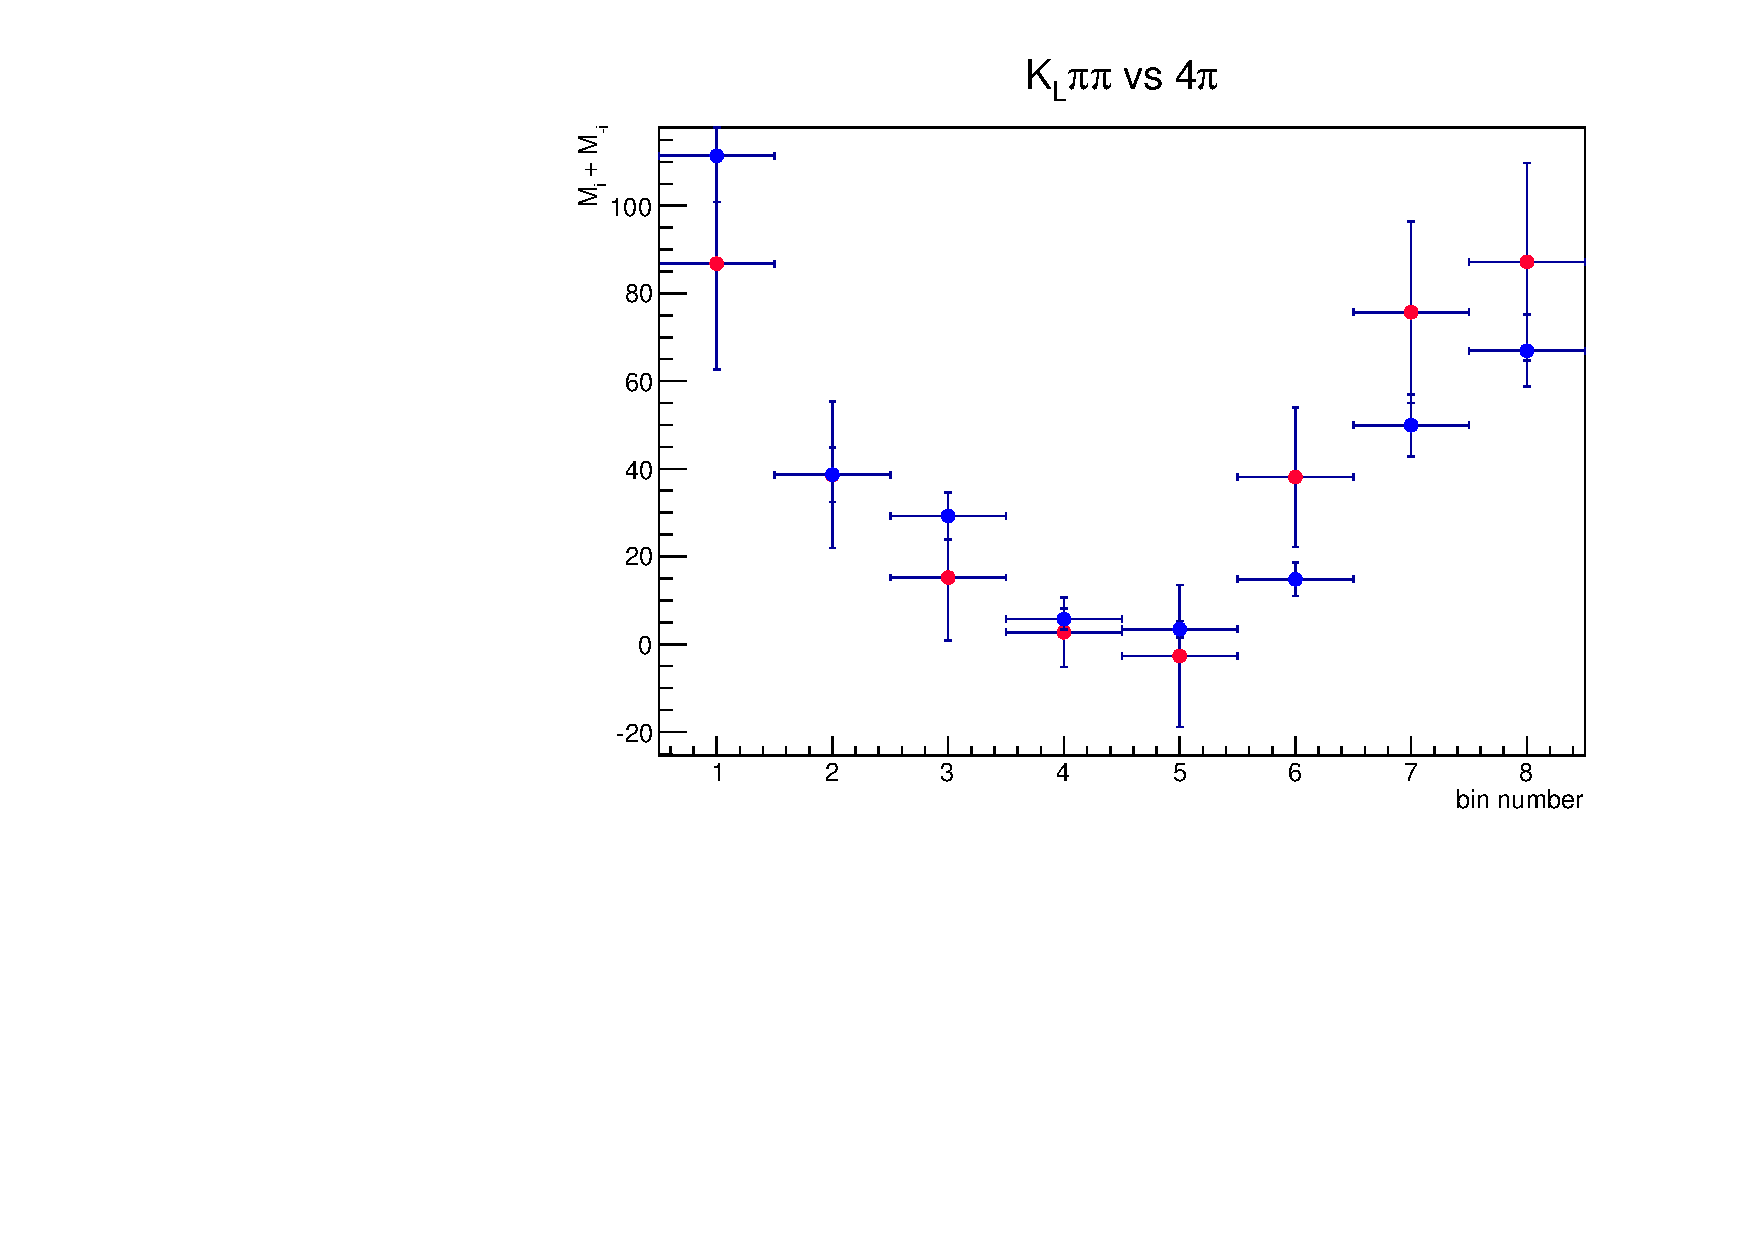
\includegraphics[width=0.48 \textwidth] {F_KKpi0_KlPiPi.pdf}}
		\vspace*{-0.5cm}
	\end{center}
	\caption{\textit{Distribution of $MM$ over the bins for $\kaon \kaon \pi^0$ vs \KsPiPi (left) and $\kaon \kaon \pi^0$ vs \KlPiPi (right). The fit was performed on both modes independently of each other. Red: data, blue: fit values. }}
\end{figure}\\
\begin{figure}[!h]
	\vspace*{-0.5cm}
	\begin{center}
	 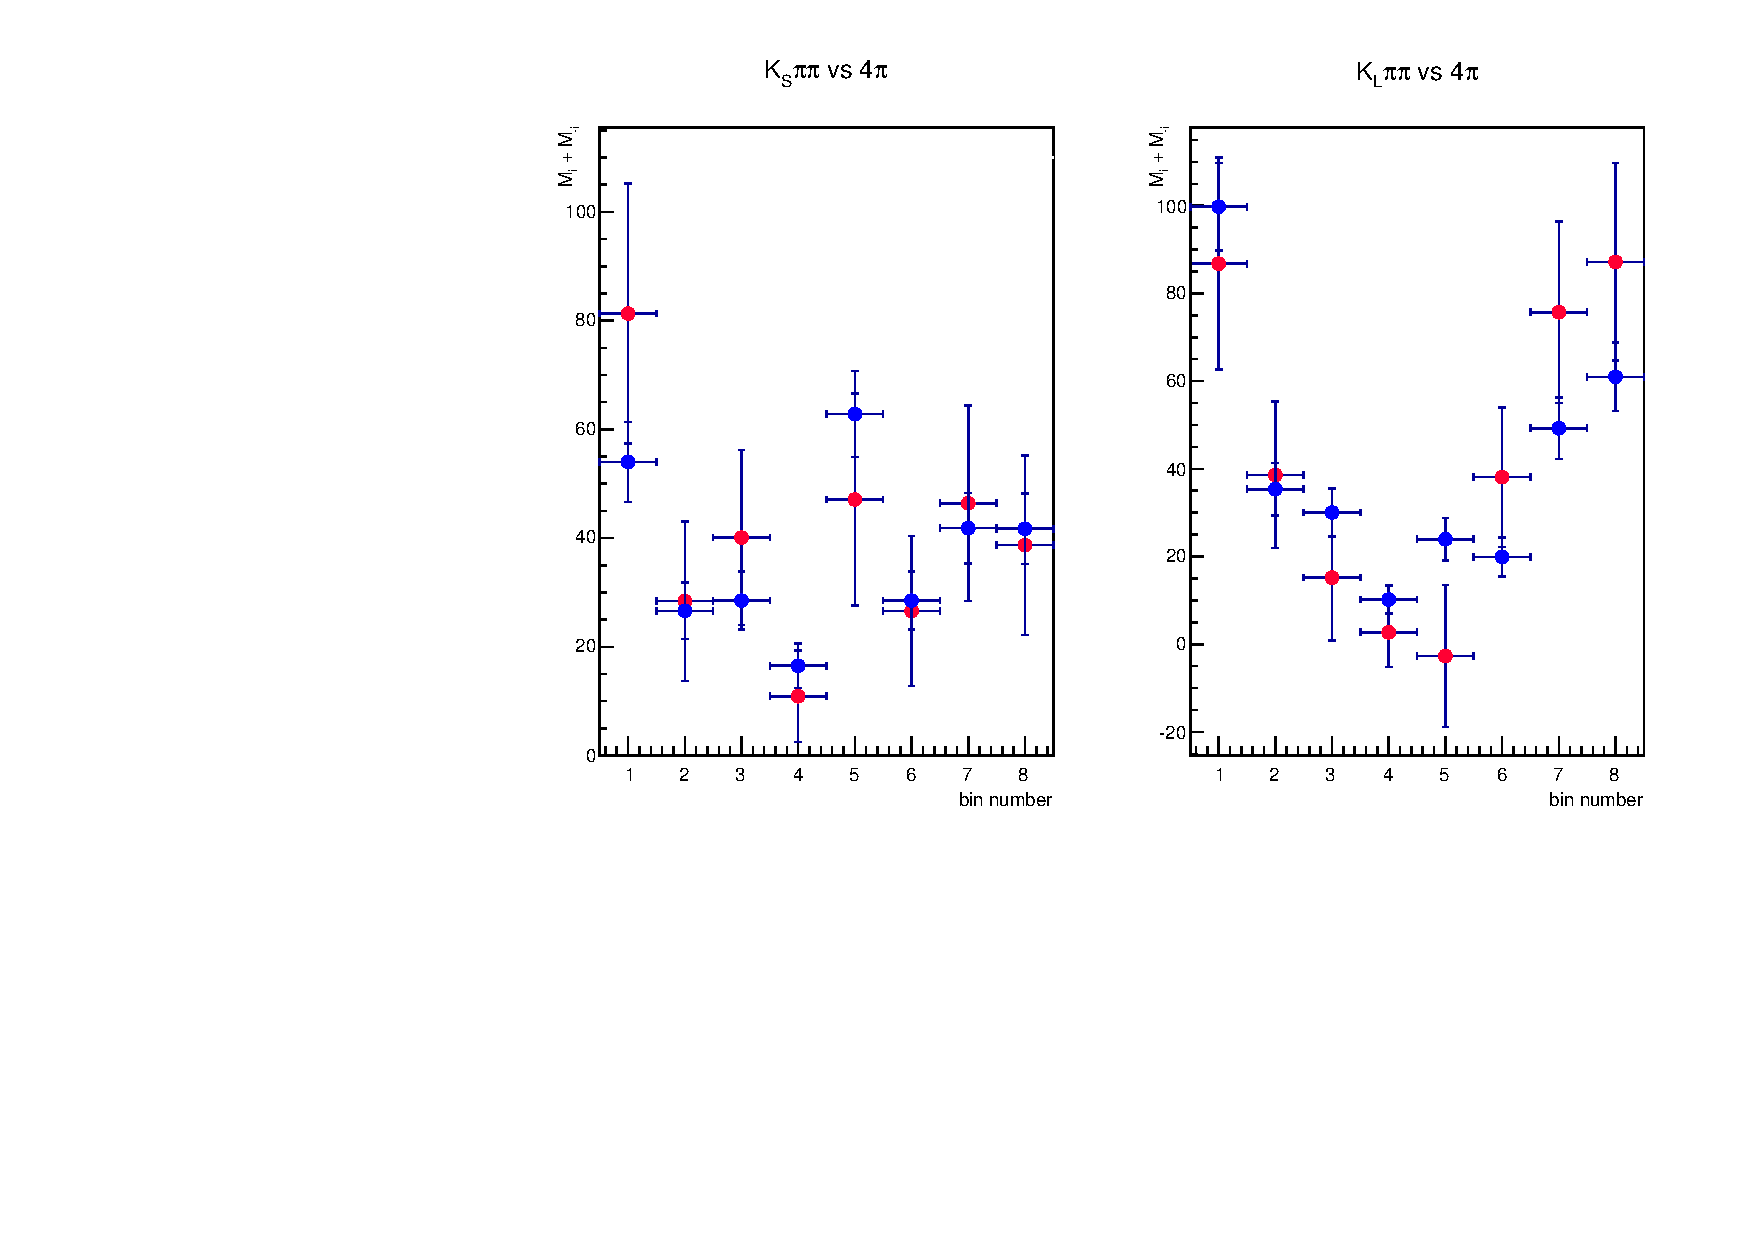
\includegraphics[width=0.96 \textwidth] {F_KKpi0_both.pdf}
		\vspace*{-0.5cm}
	\end{center}
	\caption{\textit{Distribution of $MM$ over the bins for $\pi \pi \pi^0$ vs \KsPiPi (left) and $\pi \pi \pi^0$ vs \KlPiPi (right). The fit was performed on both modes simultaneously. Red: data, blue: fit values. }}
\end{figure}\\
\clearpage
\subsection{Change in input variables}
\begin{table}[!h]
	\begin{center}
		\begin{tabular}{c| c| c|c}
			input variable & \quad shift [\%] \quad & shift/$\sigma_{fit}$ & \quad $\sigma_{fit}/ \sigma_{input}$\\
			\hline
			\hline
$c_1$ & -0.0027 & -0.00094 & 0.35\\ 
$c_2$ & 0.0041 & 0.00067 & 0.34\\ 
$c_3$ & -0.25 & -0.0016 & 0.24\\ 
$c_4$ & -0.033 & 0.0035 & 0.35\\ 
$c_5$ & -0.0069 & 0.0028 & 0.36\\ 
$c_6$ & -0.0024 & 0.0004 & 0.3\\ 
$c_7$ & 0.015 & 0.00027 & 0.33\\ 
$c_8$ & 0.016 & 0.002 & 0.33\\ 
$T_1$ & 0.065 & 0.021 & 1\\ 
$T_2$ & -0.0088 & -0.0066 & 1\\ 
$T_3$ & 0.071 & 0.026 & 1\\ 
$T_4$ & -0.057 & -0.014 & 1\\ 
$T_5$ & -0.0048 & -0.0018 & 1\\ 
$T_6$ & 0.0084 & 0.0046 & 1\\ 
$T_7$ & 0.0079 & 0.0055 & 1\\ 
$T_8$ & -0.039 & -0.024 & 1\\ 
$T_{-1}$ & 0.0089 & 0.0051 & 1\\ 
$T_{-2}$ & -0.0011 & -0.001 & 1\\ 
$T_{-3}$ & 0.0066 & 0.0042 & 1\\ 
$T_{-4}$ & -0.17 & -0.018 & 1\\ 
$T_{-5}$ & -0.003 & -0.0012 & 1\\ 
$T_{-6}$ & 0.0029 & 0.0014 & 1\\ 
$T_{-7}$ & 0.0042 & 0.0014 & 1\\ 
$T_{-8}$ & -0.037 & -0.01 & 1\\ 
\end{tabular}
\end{center}
\caption{\textit{Amount by which the Gaussian constraint input variables are shifted in the fit with the \KsPiPi mode only.}}
\end{table} 
\clearpage
\begin{table}[!h]
	\begin{center}
		\begin{tabular}{c| c| c|c}
			input variable & \quad shift [\%] \quad & shift/$\sigma_{fit}$ & \quad $\sigma_{fit}/ \sigma_{input}$\\
			\hline
			\hline	
$c'_1$ & -0.17 & -0.053 & 0.38\\ 
$c'_2$ & 0.02 & 0.0032 & 0.39\\ 
$c'_3$ & -2.7 & -0.11 & 0.47\\ 
$c'_4$ & 0.54 & -0.03 & 0.46\\ 
$c'_5$ & 0.18 & -0.042 & 0.47\\ 
$c'_6$ & -3.5 & 0.11 & 0.46\\ 
$c'_7$ & 2.3 & 0.15 & 0.48\\ 
$c'_8$ & 0.38 & 0.064 & 0.39\\ 
$T'_1$ & -0.17 & -0.068 & 1\\ 
$T'_2$ & -0.0084 & -0.0019 & 1\\ 
$T'_3$ & -0.3 & -0.061 & 1\\ 
$T'_4$ & -0.1 & -0.013 & 1\\ 
$T'_5$ & -0.0076 & -0.0021 & 1\\ 
$T'_6$ & 0.14 & 0.04 & 1\\ 
$T'_7$ & 0.14 & 0.056 & 1\\ 
$T'_8$ & 0.1 & 0.043 & 1\\ 
$T'_{-1}$ & -7.4 & -0.4 & 0.99\\ 
$T'_{-2}$ & -0.07 & -0.0034 & 0.99\\ 
$T'_{-3}$ & -2.8 & -0.15 & 0.99\\ 
$T'_{-4}$ & -0.46 & -0.022 & 1\\ 
$T'_{-5}$ & 0.21 & 0.0085 & 0.99\\ 
$T'_{-6}$ & 1.1 & 0.049 & 1\\ 
$T'_{-7}$ & 1.5 & 0.1 & 0.99\\ 
$T'_{-8}$ & 4.5 & 0.2 & 0.97\\ 
\end{tabular}
\end{center}
\caption{\textit{Amount by which the Gaussian constraint input variables are shifted in the fit with the \KlPiPi mode only.}}
\end{table} 

\clearpage
\begin{table}[!h]
	\begin{center}
		\begin{tabular}{c| c| c|c}
			input variable & \quad shift [\%] \quad & shift/$\sigma_{fit}$ & \quad $\sigma_{fit}/ \sigma_{input}$\\
			\hline
			\hline
$c_1$ & -0.097 & -0.036 & 0.32\\ 
$c_2$ & 0.026 & 0.0048 & 0.3\\ 
$c_3$ & -5 & -0.033 & 0.22\\ 
$c_4$ & 0.22 & -0.025 & 0.32\\ 
$c_5$ & 0.053 & -0.023 & 0.34\\ 
$c_6$ & 0.026 & -0.0044 & 0.28\\ 
$c_7$ & -0.77 & -0.015 & 0.32\\ 
$c_8$ & -0.033 & -0.0045 & 0.31\\ 
$c'_1$ & -0.1 & -0.034 & 0.36\\ 
$c'_2$ & 0.022 & 0.0039 & 0.34\\ 
$c'_3$ & -1.4 & -0.059 & 0.44\\ 
$c'_4$ & 0.78 & -0.045 & 0.45\\ 
$c'_5$ & 0.28 & -0.064 & 0.46\\ 
$c'_6$ & -1.2 & 0.039 & 0.44\\ 
$c'_7$ & 1.2 & 0.077 & 0.5\\ 
$c'_8$ & 0.23 & 0.039 & 0.38\\ 
$T_1$ & 0.19 & 0.062 & 1\\ 
$T_2$ & 0.0036 & 0.0026 & 1\\ 
$T_3$ & 0.073 & 0.027 & 1\\ 
$T_4$ & -0.14 & -0.033 & 1\\ 
$T_5$ & -0.11 & -0.041 & 1\\ 
$T_6$ & -0.0072 & -0.0039 & 1\\ 
$T_7$ & 0.011 & 0.0078 & 1\\ 
$T_8$ & -0.011 & -0.0066 & 1\\ 
$T_{-1}$ & 0.018 & 0.011 & 1\\ 
$T_{-2}$ & 0.00025 & 0.00023 & 1\\ 
$T_{-3}$ & 0.0067 & 0.0043 & 1\\ 
$T_{-4}$ & -0.5 & -0.052 & 1\\ 
$T_{-5}$ & -0.063 & -0.026 & 1\\ 
$T_{-6}$ & -0.0031 & -0.0015 & 1\\ 
$T_{-7}$ & 0.0046 & 0.0015 & 1\\ 
$T_{-8}$ & -0.0067 & -0.0018 & 1\\ 
$T'_1$ & -0.081 & -0.033 & 1\\ 
$T'_2$ & 0.053 & 0.012 & 1\\ 
$T'_3$ & -0.34 & -0.07 & 1\\ 
$T'_4$ & -0.44 & -0.057 & 1\\ 
$T'_5$ & -0.22 & -0.06 & 1\\ 
$T'_6$ & 0.14 & 0.04 & 1\\ 
$T'_7$ & 0.15 & 0.06 & 1\\ 
$T'_8$ & 0.13 & 0.054 & 1\\ 
$T'_{-1}$ & -3.2 & -0.17 & 0.99\\ 
$T'_{-2}$ & 0.56 & 0.027 & 0.99\\ 
$T'_{-3}$ & -2.9 & -0.15 & 0.99\\ 
$T'_{-4}$ & -2.2 & -0.1 & 0.99\\ 
$T'_{-5}$ & -5.1 & -0.21 & 0.99\\ 
$T'_{-6}$ & 1.6 & 0.066 & 1\\ 
$T'_{-7}$ & 1.2 & 0.086 & 1\\ 
$T'_{-8}$ & 4.6 & 0.2 & 0.98\\ 
\end{tabular}
\end{center}
\caption{\textit{Amount by which the Gaussian constraint input variables are shifted in the fit with the \KsPiPi and \KlPiPi mode simultaneously.}}
\end{table} 
